%
% Documento: Fundamentação Teorica
%

%\vspace{3cm}%Espaçamento entre linhas

\chapter{\textbf{FUNDAMENTAÇÃO TEÓRICA}}\label{chap:fundTeorica}

Le présent travail propose de développer un système web, qui vise à gérer les animaux, fournissant ainsi un contrôle des médicaments, ainsi que l'application d'un contrôle du poids.

\section{TRABALHOS RELACIONADOS}


Durante o levantamento de dados foram buscadas plataformas que trabalham de forma semelhante ao presente sistema, como por exemplo o BovControl, o JetBov e o A3Pecuária, que serão apresentadas a seguir.

\subsection{BOVCONTROL}

BovControl é uma ferramenta de coleta e análise de dados provenientes da pecuária para melhorar a performance da produção de carne, leite ou genética \cite{bovcontrol10}.

É disponibilizado em forma de aplicativo e possui um plano gratuito, no qual é possível gerir um rebanho e faz os seguintes manejos nos animais: saída, lote, exame de toque, controle reprodutivo, idade da cria, idade do desmame, medicamento, origem, pesagem, perímetro escrotal, leite, teste diagnóstico, tipo de entrada, vacina, vermifugação. Também é possível visualizar seus dados em um dashboard\footnote{"Dashboards são painéis que mostram métricas e indicadores importantes para alcançar objetivos e metas traçadas de forma visual, facilitando a compreensão das informações geradas." \cite{nascimento17}.}. na internet.

Possui uma parte de relatórios com apenas 2 gráficos, um do total de animais e do tipo de produção do animal (como leite, engorda e genética), e outro do total de animais e do gênero (macho ou fêmea).

Possui 3 planos profissionais que variam de R\$ 22,99 a R\$ 32,99 por mês. Estes planos incluem gestor financeiro, gestor de tarefas, multiusuários, relatórios personalizados, importação de animais por planilha e estoque de maquinário.

A Figura 1, é uma imagem mostrando a página inicial do sistema BovControl versão web.

\begin{figure}[H]
	\begin{center}
		\caption{Dashboard do BovControl}
		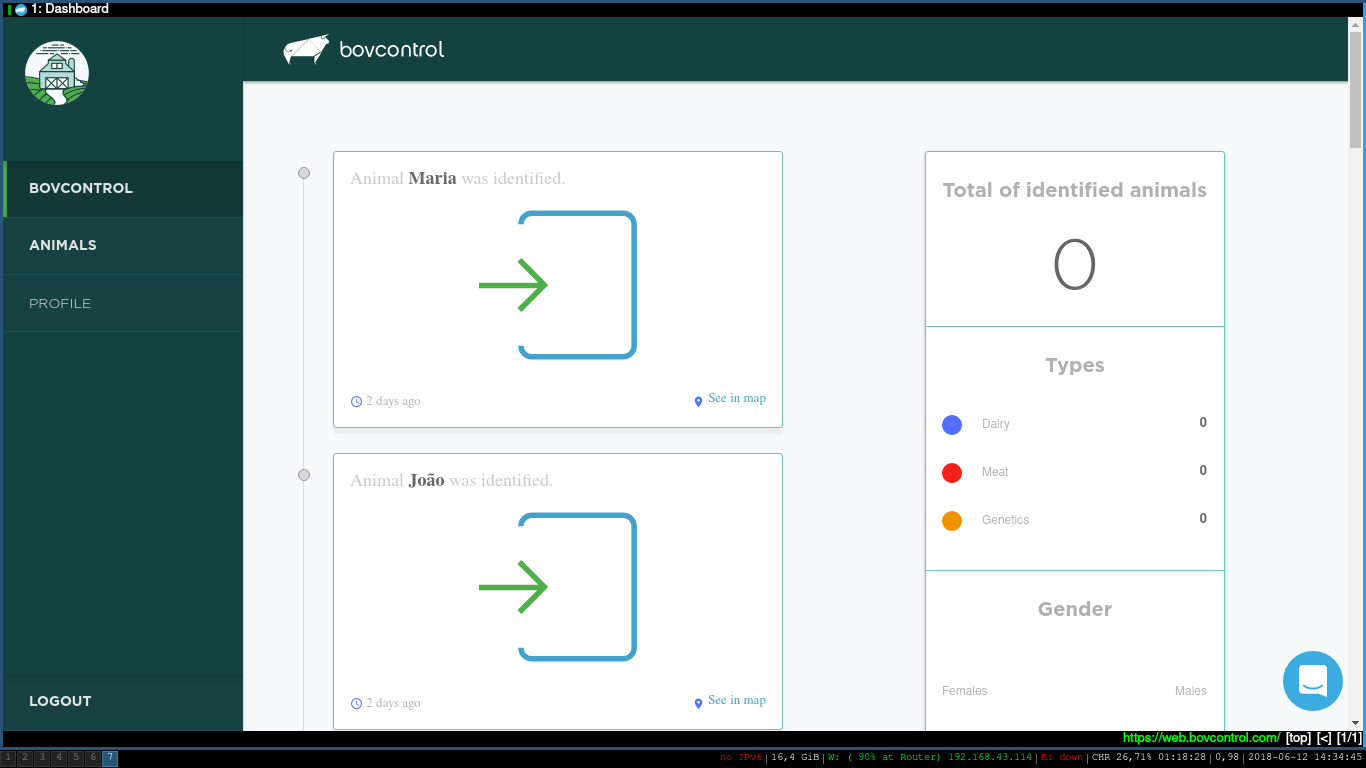
\includegraphics[width=6in]{../img/bovcontrol.png}

		Fonte: Captura de tela do sistema BovControl.
	\end{center}
\end{figure}


%\begin{figure}[!h]
%\begin{center}
%\caption{BovControl versão mobile - Página inicial}
%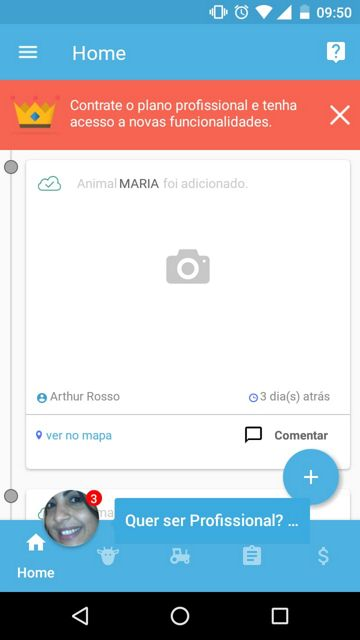
\includegraphics[width=6in]{img/bovcontrolapp1.jpg}

% % %\floatfoot{Fonte: Autoria própria.}
%\end{center}
%\end{figure}

%\begin{figure}[!h]
%\begin{center}
%\caption{BovControl versão mobile - Opções de ações}
%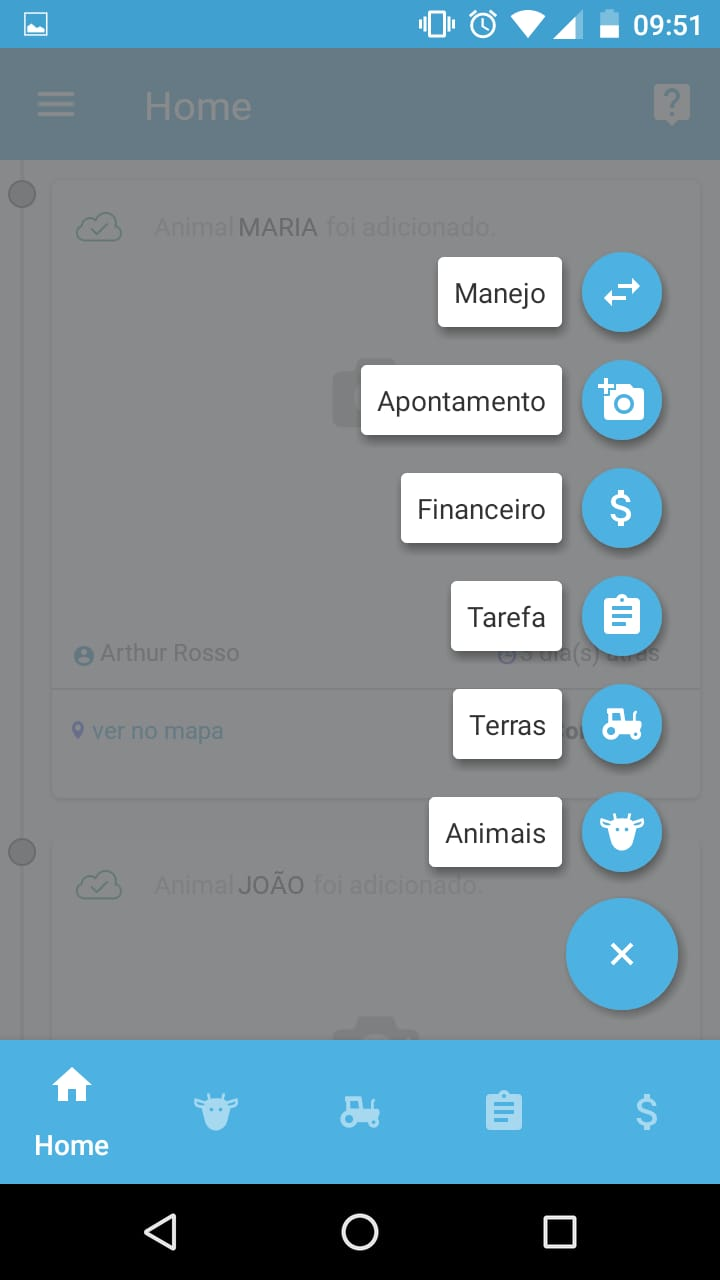
\includegraphics[width=6in]{img/bovcontrolapp2.jpeg}

% %\floatfoot{Fonte: Autoria própria.}
%\end{center}
%\end{figure}


\subsection{JETBOV}

Segundo \citeonline{jetbov16}, esse é um sistema que tem como objetivo a gestão da fazenda, da cria até a terminação, a pasto, no semi-confinamento ou confinamento, com um controle de custos com o propósito de aumento da rentabilidade.

Não possui versão gratuita, porém há uma versão de testes disponível por 21 dias, após isso é necessário realizar um orçamento individual.

O sistema apresenta 2 versões, uma web e outra mobile, a mobile é simples contendo apenas uma página com animais e um botão contendo as opções de manejo como adicionar um novo animal e sua identificação, registros sanitários como vacinações, medicações, exames, vermifugações, etc, adicionar a morte de um animal, o desmame, o parto e pesagem.

A versão web é mais completa contendo um painel de dados da fazenda, com gráficos de animais por sexo, animais por lote, peso por lote e algumas informações como número total de animais da fazenda, peso total da fazenda.

A Figura 2 apresenta uma imagem mostrando a página inicial do sistema JetBov versão web.

\begin{figure}[H]
	\begin{center}
		\caption{Página inicial da versão web do JetBov}
		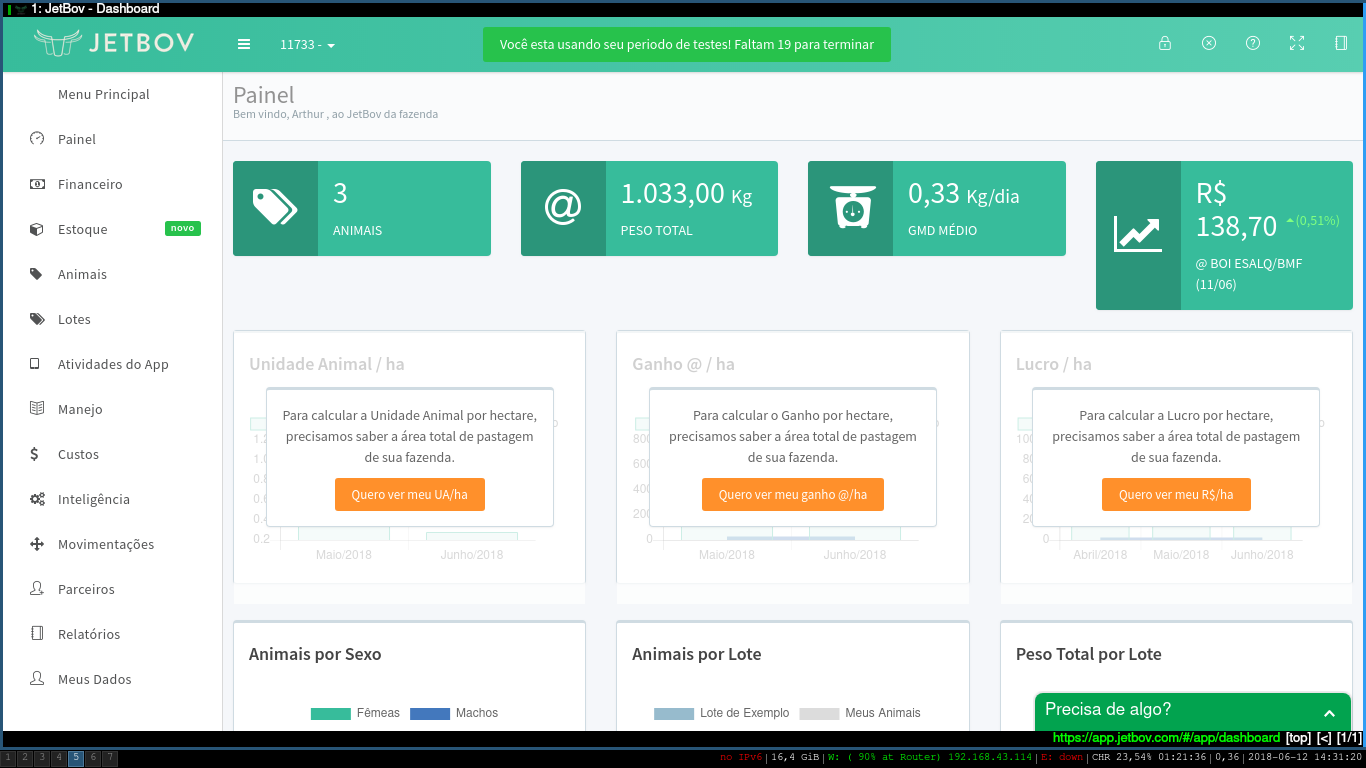
\includegraphics[width=6in]{../img/jetbov.png}

		Fonte: Captura de tela do sistema JetBov.
	\end{center}
\end{figure}

%\begin{figure}[!h]
%\begin{center}
%\caption{Jetbov versão mobile - Página inicial}
%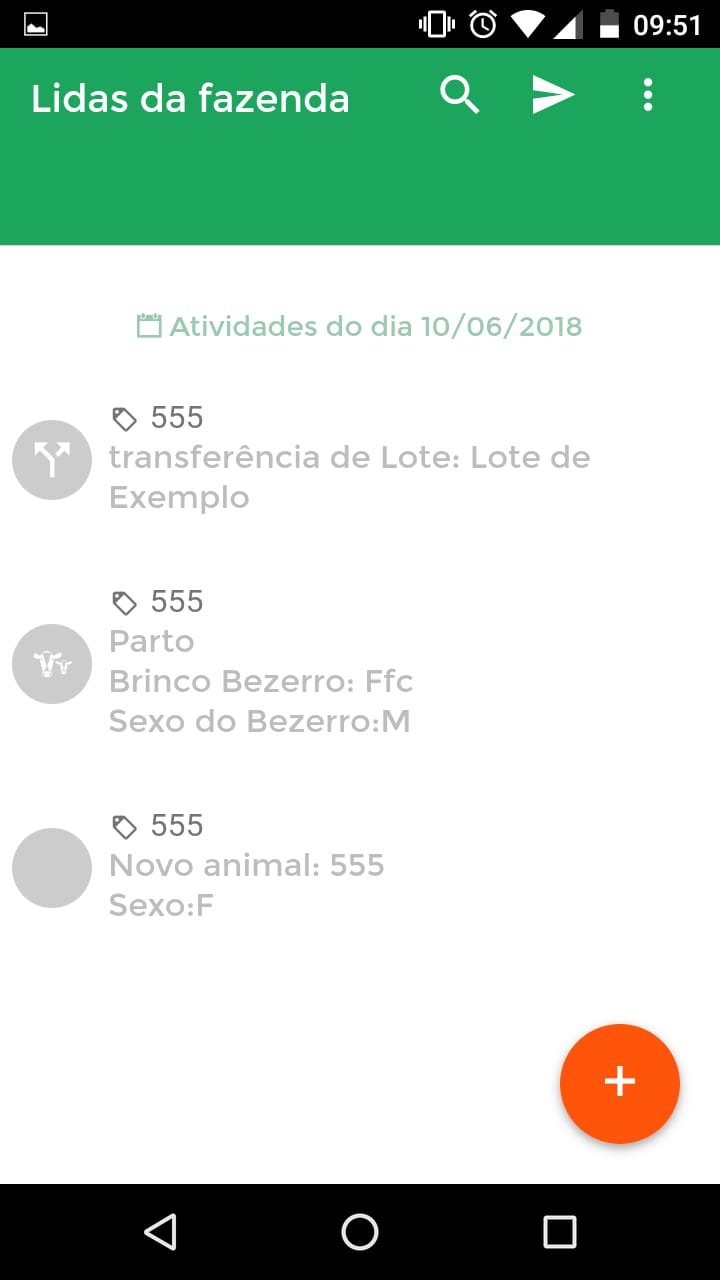
\includegraphics[width=6in]{img/jetbovapp1.jpeg}

% %\floatfoot{Fonte: Autoria própria.}
%\end{center}
%\end{figure}

%\begin{figure}[!h]
%\begin{center}
%\caption{JetBov versão mobile - Opções de ações}
%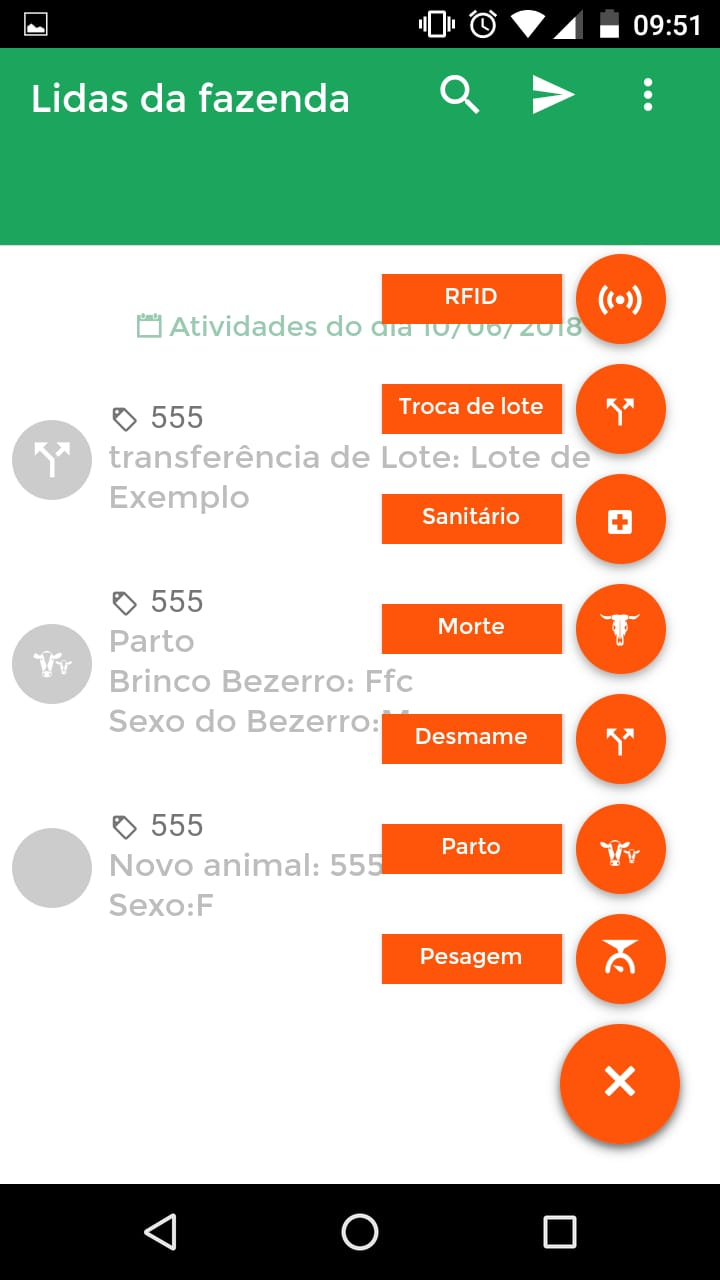
\includegraphics[width=6in]{img/jetbovapp2.jpeg}

% %\floatfoot{Fonte: Autoria própria.}
%\end{center}
%\end{figure}

\subsection{A3PECUÁRIA}

A3Pecuária é um software para gestão de animais com controle de reprodução, pesagens, vacinas e exames, controle financeiro e de estoque e compra e venda. Segundo o site do fabricante: "fornecemos importantes informações de análise de seu rebanho de maneira simples e com uma interface muito fácil de aprender, permitindo gerir seu investimento de forma a aumentar a lucratividade"  \cite{a3pecuaria16}.

Segundo \citeonline{a3pecuaria16}, são 3 tipos de planos, que variam de R\$ 29,90 a R\$ 69,90 por mês, e que gerenciam 500 animais ativos e 1 Fazenda até 3000 animais ativos e fazendas ilimitadas. Não possui versão gratuita, mas uma versão de testes por 30 dias.

Apresenta duas versões, uma web e outra mobile. A mobile, por ser simples, contém apenas a lista de animais da fazenda, o inventário, uma opção de bastão eletrônico e links para a versão web.

A versão web, por ser mais robusta e completa, apresenta uma série de possibilidades de manejos como novo lote, novo animal, nova despesa, nova receita e uma série de análise de dados com relatórios da propriedade.

A seguir, uma imagem mostrando a página inicial do sistema A3Pecuária versão web.


\begin{figure}[!h]
	\begin{center}
		\caption{Página inicial da versão web do A3Pecuária}
		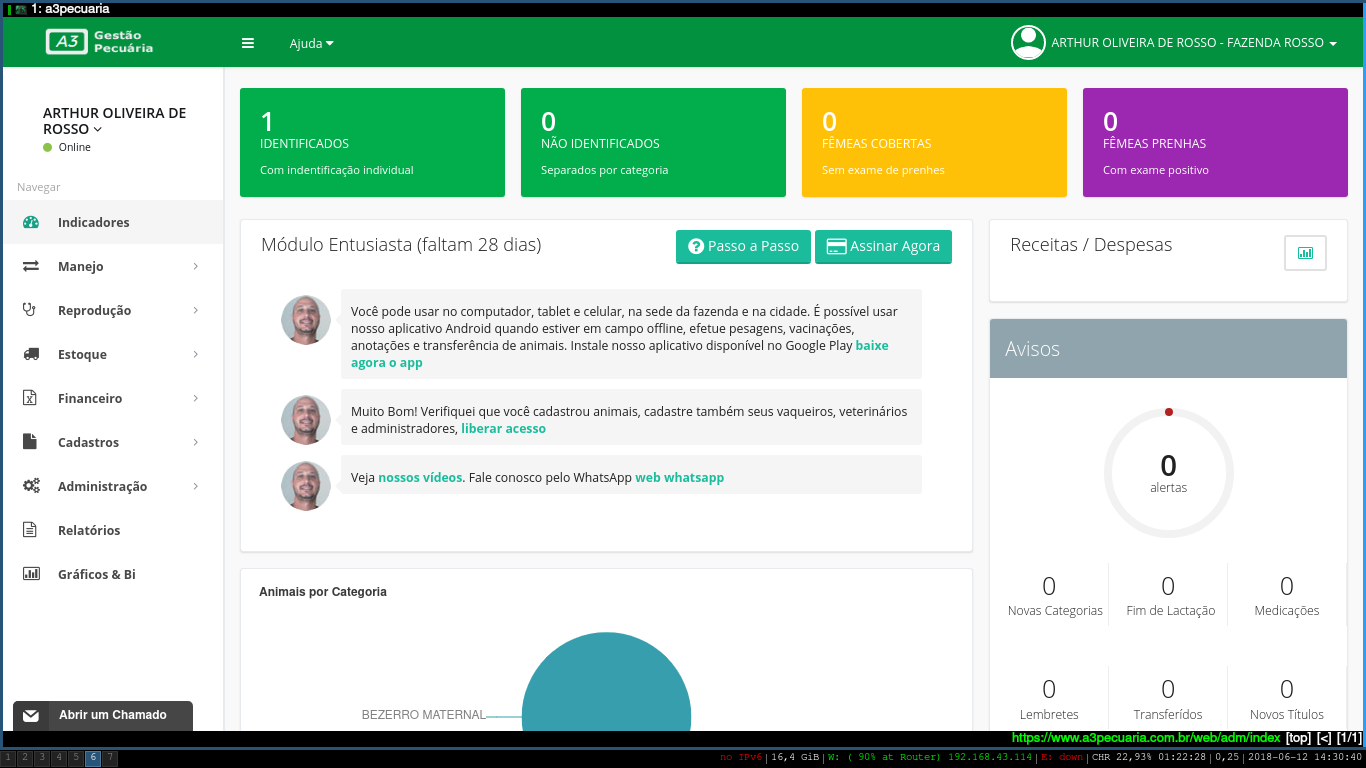
\includegraphics[width=6in]{../img/a3pecuaria.png}

		Fonte: Captura de tela do sistema A3Pecuária.
	\end{center}
\end{figure}

%\begin{figure}[!h]
%\begin{center}
%\caption{A3Pecuária versão mobile - Página inicial}
%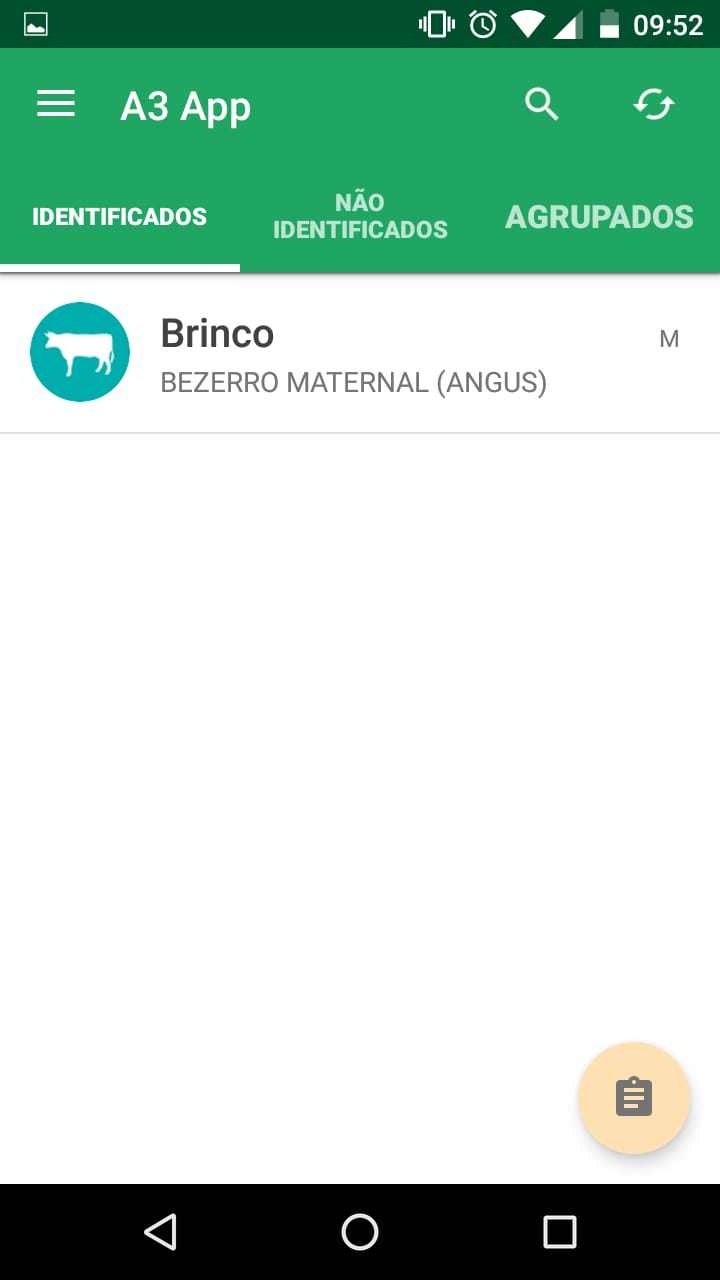
\includegraphics[width=6in]{img/a3pecuariaapp1.jpeg}

% %\floatfoot{Fonte: Autoria própria.}
%\end{center}
%\end{figure}

%\begin{figure}[!h]
%\begin{center}
%\caption{A3Pecuária versão mobile - Opções de ações}
%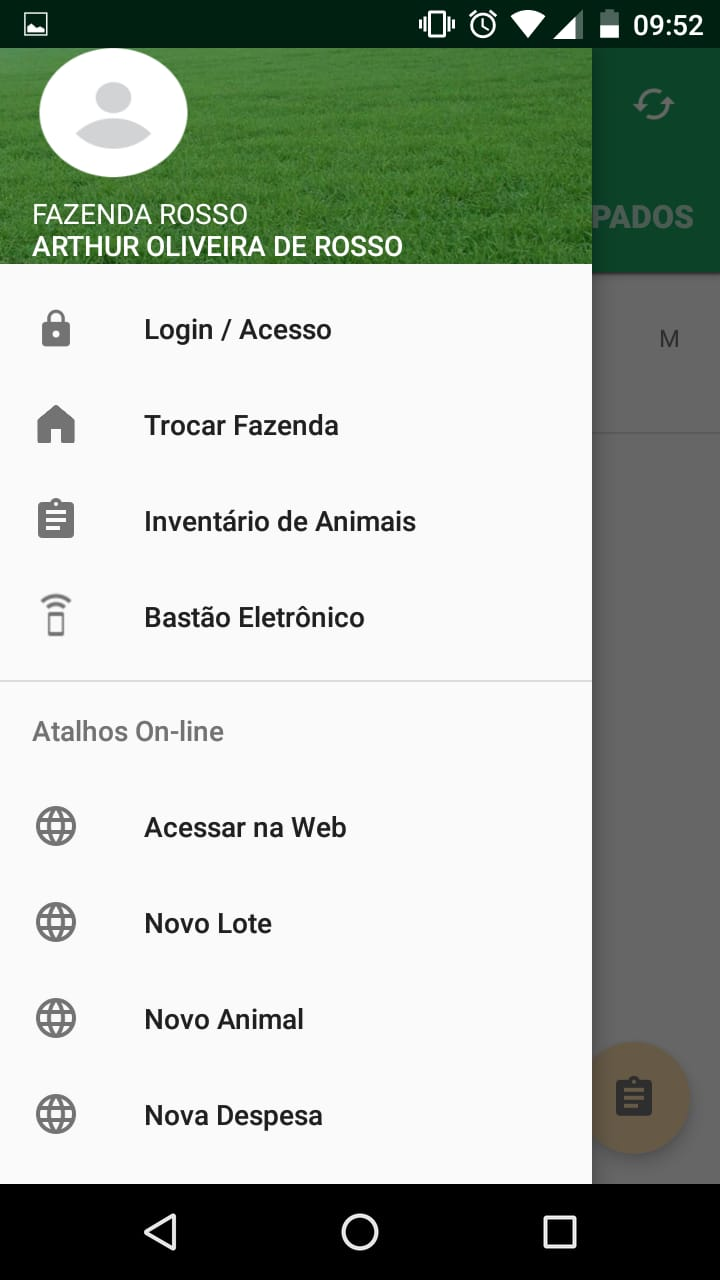
\includegraphics[width=6in]{img/a3pecuariaapp2.jpeg}

% %\floatfoot{Fonte: Autoria própria.}
%\end{center}
%\end{figure}

\subsection{ANÁLISE COMPARATIVA DOS TRABALHOS RELACIONADOS}

A partir da análise feita nas plataformas, pode-se chegar na seguinte conclusão: todas tem seu modo de operação semelhante, como criar, deletar, ler e editar as informações de um animal, e as opções de tratamento de gado (aqui chamado de manejo). As opções de estoque, que no proposto sistema é trabalhado só com medicações e a visualização de relatórios são trabalhados de maneira parecida em todos os sistemas. Dessa maneira o presente sistema tem por objetivo trabalhar com estas mesmas operações, de maneira simples e sem custos.
\begin{table}[H]
	\begin{center}
		\caption{Tabela da análise dos trabalhos relacionados}
		\begin{tabular}{ | p{8cm} |  c | c | c | c |}
			\hline
			Funcionalidade & BovControl & JetBov & A3Pecuária & GoBov \\ \hline
			Gerenciamento de animais de uma propriedade & Sim & Sim & Sim & Sim \\  \hline
			Gerenciamento de medicamentos de uma propriedade & Não & Não & Sim & Sim  \\ \hline
			Gerenciamento de medicações de animais & Sim & Sim & Sim & Sim  \\ \hline
			Visualização de relatórios gerais da propriedade & Sim & Sim & Sim & Sim  \\ \hline
			Visualização de relatórios individuais de cada animal & Não & Não & Não & Sim  \\ \hline
			Versão gratuita & Sim & Não & Não & Sim  \\
			\hline
		\end{tabular}
		Fonte: Autoria própria.
	\end{center}
\end{table}


\section{TECNOLOGIAS UTILIZADAS}

Esta seção tratará as tecnologias que foram utilizadas na produção do presente trabalho.

A linguagem utilizada no \textit{back-end} é Go, uma linguagem de programação de código aberto que facilita a criação de software simples, bastante adequada para um TCC.

Foi utilizado o banco de dados MariaDB, trata-se de um banco de dados de código aberto bastante conhecido, é um \textit{fork} do MySQL.

Para a construção do \textit{front-end} foi utilizada a linguagem de marcação HTML que providencia a estrutura da página, para os estilos CSS. JavaScript, que é uma linguagem de programação que executa scripts no lado do cliente também foi utilizada. Também se utilizou o framework Materialize, como um facilitador da estilização das páginas HTML, assim foi possível deixa-las responsivas.
